\documentclass[12pt]{article}
\usepackage{graphicx}
\usepackage{pst-xkey}
\usepackage[spanish]{babel}
%opening


\author{Victor Hugo Pacheco Fonseca}

\begin{document}
	
	\title{\Huge{\textbf{HULK }}\\
		{\Large{{(Havana University Language for Kompilers)}}}}
	
	
	\author{\textit{Victor Hugo Pacheco Fonseca}}
	\date{8 de octubre del 2023}
	
	
	\maketitle
	\newpage
	
	\section{\Huge {Introducción}}	
	HULK es un lenguaje de programación imperativo, funcional, estática y fuertemente tipado. Casi todas las instrucciones en HULK son expresiones. En este proyecto se implementó un subconjunto de este  que se compone solamente de expresiones que pueden escribirse en una línea.
	
	
	\newpage
	\section{\Huge {Que puede hacer}}	
	\subsection{Expresiones básicas}
	Todas las expresiones en Hulk deben terminar en ;. Cuenta con las constantes matemáticas  PI y E , además de los operadores matemáticos básicos:
	
	\begin{center}
		\begin{figure}[h!]
			\centering
			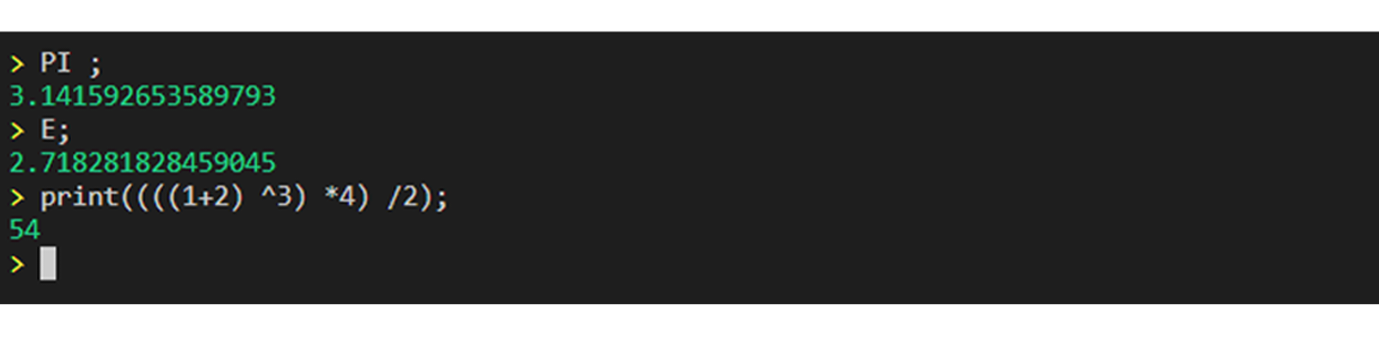
\includegraphics[scale=0.3]{imagen4}
		\end{figure}
	\end{center}
	
	
	Además cuenta con funciones matemáticas tales como:
	sin(x), cos(x), log(x,y) ,sqrt(x), pow(x,y) y rand() ,donde  sin y cos reciben su parámetro en radiales.\\
	Los string en Hulk también esta definidos y deben ir entre doble comillas. Estos puede ser concatenados con otros string (o la representación en string de números)  a traves del operador @.
	
	
	\subsection{Funciones}
	En Hulk se pueden declarar funciones inline. Las cuales
	puede ser definidas de la siguiente forma:
	\textit{function} name(operadores) $\Rightarrow$ \textit{cuerpo} \textit{de} \textit{la} \textit{funcion}};
	Estas funciones pueden ser simples,compuestas y recursivas.
	\begin{center}
		\begin{figure}[h!]
			\centering
			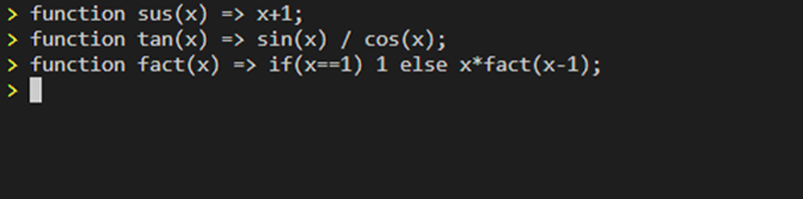
\includegraphics[scale=0.3]{imagen5}
		
		\end{figure}
	\end{center}
	\subsection{Variables}
	En Hulk es posible declarar variables usando la expresion let-in, mediante la sintaxis: \textit{let} identifier = value \textit{in} expression ;\\
	En general, una expresion let-in consta de una o mas delaraciones de variables, y fuera de la expresión let-in dejan de existir.
	\begin{center}
		\begin{figure}[h!]
			\centering
			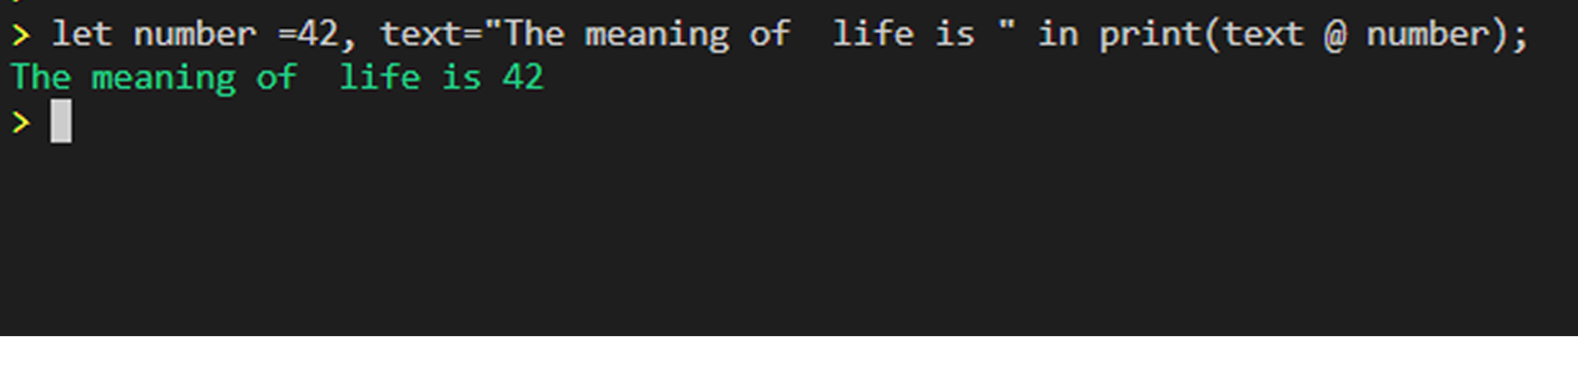
\includegraphics[scale=0.3]{imagen6}
		\end{figure}
	\end{center}
	
	\subsection{Condicionales}
	Las condiciones en Hulk se implemetan mediante una expresión if-else, que debe recibir una expresión boleana entre parentesis, y dos expresiones para el cuerpo de if y del else(siempre ambas partes).
	\begin{center}
		\begin{figure}[h!]
			\centering
			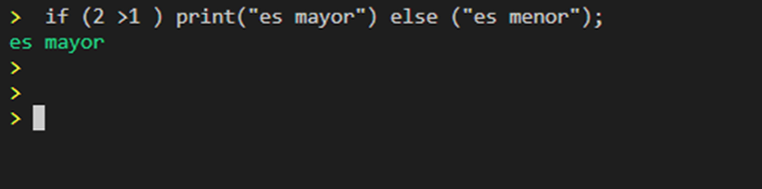
\includegraphics[scale=0.4]{imagen7}
			
		\end{figure}
	\end{center}
	
	\section{\Huge {Funcionamiento}}
	\subsection{ \Large{Lexer}}
	La primera fase del compilador es el analizador léxico.Durante esta etapa el código fuente  se divide en unidades léxicas llamadas tokens, estos representan componentes básicos del lenguaje : palabras reservadas, identificadores, números, strings y operadores. El encargado  de esto es la clase Lexer, con su método Scanner. Su objetivo es identificar los diferentes tokens, crear un objeto de tipo Token donde se almacena su valor, posición y tipo, para luego almacenarlos en una lista.  \\
	\subsubsection{Tipos de tokens}
	Los tokens se clasifican en :
	\begin{enumerate}
		\item NumberToken
		\item StringToken
		\item PlusToken	
		\item MinusToken
		\item MultiplicationToken
		\item DivisionToken
		\item RestoToken
		\item ExponentToken
		\item ArrobaToken
		\item AndOperatorToken
		\item OrOperatorToken
		\item NotOperatorToken
		\item EqualEqualToken
		\item NotEqualToken
		\item ComparisonToken
		\item AssignmentToken
		\item OpenParenthesesToken
		\item CloseParenthesesToken
		\item ReservedWordToken
		\item ReservedFunctionToken
		\item IdentifierToken
		\item ColonToken
		\item SemiColonToken
		\item EndLineToken
	\end{enumerate}
	
	
	\subsection{{Parser}}
	La segunda fase del compilador es el análisis sintáctico, también conocido como parsing. Este recibe la lista de tokens del Lexer y verifica que se cumplan las reglas sintácticas establecidas y se construye una estructura de datos (árbol sintáctico) que representa la sintáxis del programa. De esto se encarga la clase Parser, en la cual se encuentran diversos métodos que retornan un objeto tipo Expression (clase de la cual heredan muchas otras ) donde cada uno revisa un operador diferente, y de forma tal que los métodos que verfican operadores de mayor precedencia se llamen dentro de los de menor precedencia, asegurandose asi que en la creación del árbol un nodo (operador) de menor precedencia siempre esta arriba de uno de mayor precedencia.\\
	Por ejemplo para el codigo 2*3+1 :\\
	Pirmero se llama al metodo ParseTerm()  el cual verifca los operadores '+' y '-', pero antes llama al metodo ParseProduc() que verifica si hay alguno de los operadores '*' y '/' , y retorna un objeto tipo BinaryExpression que hereda de la clase Expression , que no es mas que una estructura de datos donde tiene un nodo el cual es un Token operador, y dos campos de clases de tipo Expression, left y right, en este caso retornaria BinaryExpression(2 , * , 3).Hecho  esto la funcion ParseTerm() identifica el siguente token '+' y retorna un objeto tipo BinaryExpression donde se almacena el arbol sintactico correspondiente.
	
	
	\subsection{\textit{Evaluator}}
		Terminado el análisis sintáctico, la tercera fase es el análisis semántico, el cual verificar que no halla errores semánticos como por ejemplo una suma de expresiones que no sean tipo números  .De esto se encarga la clase Execute, el método Evaluator(). Dicho método evalua recursivamante el árbol sintáctico mientras va  desciendiendo en él.
	

	

	
	
\end{document}
